\section{DMA \weekDoran{3}}
	\subsection{Operation Modes}
			\begin{longtable}{|p{0.3\linewidth}|p{0.65\linewidth}|}
				\hline
				\textbf{Burst Mode}
					& Contiguous block is transferred in one. System bus and/or memory is solely reserved by the DMA.\\
				\hline
				\textbf{Cycle Stealing Mode}
					& Continually requesting and yielding control of the bus/resource. Causes the transfer to take longer in general.\\
				\hline
				\textbf{Transparent Mode}
					& CPU never waits for the resource, and DMA only transfers when the CPU doesn't need the bus.\\
				\hline	
				\textbf{Flyby Mode}
					& Transfers data in one cycle rather than the read/write cycle. Isn't supported by many controllers.\\
				\hline
			\end{longtable}
	\subsection{Scatter-Gather}
		A scatter-gather DMA is able to collect and organize data from non contiguous addresses or can rearrange collected data. The advantage is, that some rearranging operation can be sourced out from software to hardware.
		\begin{longtable}{p{0.475\linewidth}p{0.475\linewidth}}		 			
			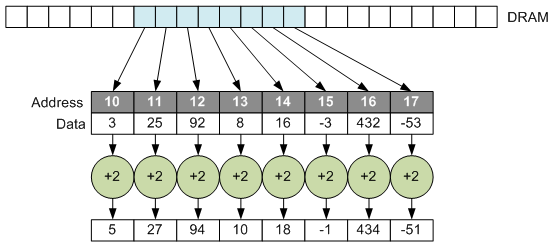
\includegraphics[width=1\linewidth]{./pictures/scatter1.png}
			& 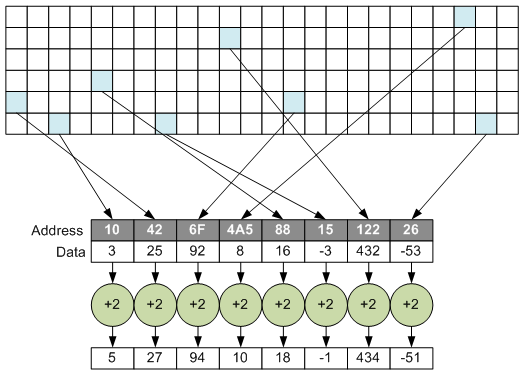
\includegraphics[width=1\linewidth]{./pictures/scatter2.png} \\
			
			Normal DMA 
			& Scatter-Gather DMA\\
		\end{longtable}